% =====================================================================
% m1.tex -- Member 1 (Cache Architecture & Storage) report sections
%   * Introduction
%   * Literature Review, subsection A (memory hierarchy, locality, mapping)
%   * Proposed Solution, subsection A (address mapping and storage)
%
% For M5: % =====================================================================
% m1.tex -- Member 1 (Cache Architecture & Storage) report sections
%   * Introduction
%   * Literature Review, subsection A (memory hierarchy, locality, mapping)
%   * Proposed Solution, subsection A (address mapping and storage)
%
% For M5: % =====================================================================
% m1.tex -- Member 1 (Cache Architecture & Storage) report sections
%   * Introduction
%   * Literature Review, subsection A (memory hierarchy, locality, mapping)
%   * Proposed Solution, subsection A (address mapping and storage)
%
% For M5: % =====================================================================
% m1.tex -- Member 1 (Cache Architecture & Storage) report sections
%   * Introduction
%   * Literature Review, subsection A (memory hierarchy, locality, mapping)
%   * Proposed Solution, subsection A (address mapping and storage)
%
% For M5: \input{sections/m1} pieces into the IEEEtran report, or copy the
% blocks marked BEGIN/END. Figure path assumes the report lives in docs/.
% Citation keys used: smith1982, hill1989, jouppi1990, hennessy2017, patterson2020
% (bibitems at the bottom of this file -- merge into the shared reference list).
% =====================================================================

% ------------------------- BEGIN INTRODUCTION -------------------------
\section{Introduction}
Processor speeds have grown far faster than main-memory access times, so a
modern CPU would spend most of its cycles waiting on DRAM without a memory
hierarchy. A cache is a small, fast memory placed between the processor and
main memory. It keeps recently used blocks close to the processor and serves
most accesses in a single cycle. This works because real programs show
\emph{temporal locality} (a recently used address is likely to be used again
soon) and \emph{spatial locality} (addresses near a recently used one are
likely to be used next)~\cite{smith1982,hennessy2017}.

This project designs and verifies a parameterised direct-mapped cache
controller in Verilog. The default configuration is a 1\,KB cache with
16-byte blocks and 32-bit byte addresses. The design is split into storage
(data, tag and valid-bit RAMs and the address decoder), control (tag
comparator and controller FSM) and a main-memory interface. It is exercised
with sequential, repeated, random and conflict-heavy address traces, and
evaluated by hit ratio, miss ratio, average memory access time (AMAT) and
synthesis cost.
% -------------------------- END INTRODUCTION --------------------------


% ---------------------- BEGIN LITERATURE REVIEW A ---------------------
\subsection{Memory Hierarchy, Locality and Mapping Schemes}
Smith's survey of cache memories~\cite{smith1982} set out the main design
choices still used today: placement policy, block size, replacement and write
policy. It showed that small caches can achieve high hit ratios because of
program locality. The survey also showed that block size is a trade-off.
Larger blocks exploit spatial locality but raise the miss penalty, and in a
small cache they increase misses because fewer blocks fit.

Placement policy decides where a memory block may live in the cache. In a
\emph{direct-mapped} cache each block has exactly one possible line, chosen
by the index bits of the address. A \emph{fully associative} cache allows any
line, and an $n$-way \emph{set-associative} cache allows any of $n$ lines in
one set. Hill and Smith~\cite{hill1989} evaluated associativity with
trace-driven simulation and classified misses as compulsory, capacity and
conflict. Direct mapping suffers most from conflict misses, because two
frequently used blocks with the same index keep evicting each other. Its
advantage is that only one tag comparison is needed and no replacement
decision has to be made. This makes the hit path short and the hardware
small, so a direct-mapped cache can have a lower hit time than an associative
cache of the same size.

Jouppi~\cite{jouppi1990} kept the fast direct-mapped hit path and attacked
its conflict misses instead, by adding a small fully associative victim
cache that holds recently evicted lines. Textbook treatments by Hennessy and
Patterson~\cite{hennessy2017,patterson2020} combine these effects into a
single metric:
\begin{equation}
\mathrm{AMAT} = t_{\mathrm{hit}} + m \cdot t_{\mathrm{penalty}},
\end{equation}
where $m$ is the miss ratio. These sources motivate the design choices in
this project: direct mapping for a single-cycle hit and simple hardware, and
conflict-heavy traces to expose its main weakness.
% ----------------------- END LITERATURE REVIEW A ----------------------


% ---------------------- BEGIN PROPOSED SOLUTION A ---------------------
\subsection{Address Mapping and Cache Storage}

\subsubsection{Address breakdown}
For a cache of $C$ bytes with blocks of $B$ bytes and an $A$-bit address, the
number of lines and the field widths are
\begin{align}
N &= C/B, & b_{\mathrm{off}} &= \log_2 B,\\
b_{\mathrm{idx}} &= \log_2 N, & b_{\mathrm{tag}} &= A - b_{\mathrm{idx}} - b_{\mathrm{off}}.
\end{align}
With $C = 1024$, $B = 16$ and $A = 32$, this gives $N = 64$ lines, a 4-bit
offset (2 word-select bits and 2 byte bits), a 6-bit index and a 22-bit tag
(Table~\ref{tab:addr}). For example, address \texttt{0x12345678} decodes to
tag \texttt{0x048D15}, index 39 and word 2.

\begin{table}[t]
\centering
\caption{Address fields for the default configuration}
\label{tab:addr}
\begin{tabular}{lccc}
\hline
Field & Bits & Width & Selects \\
\hline
Tag      & [31:10] & 22 & Block identity \\
Index    & [9:4]   & 6  & One of 64 lines \\
Word     & [3:2]   & 2  & One of 4 words \\
Byte     & [1:0]   & 2  & Unused (word access) \\
\hline
\end{tabular}
\end{table}

The \texttt{address\_decoder} module is purely combinational. Its field
widths are Verilog parameters derived from \texttt{CACHE\_SIZE},
\texttt{BLOCK\_SIZE} and \texttt{ADDR\_WIDTH}, so the same RTL can be
re-targeted for the Phase~II parameter sweep without editing code. The unit
test checks both the default configuration and a 2\,KB / 32\,B configuration
(21/6/3/2 split).

\subsubsection{Storage organisation}
The cache state is held in three structures, all indexed by the same 6-bit
index (Fig.~\ref{fig:block}):
\begin{itemize}
  \item \textbf{Data RAM:} $64 \times 128$ bits (four 32-bit words per line,
        1\,KB). It supports a full-line write for refills and a single-word
        write for write hits. If both are requested, the line write takes
        priority.
  \item \textbf{Tag RAM:} $64 \times 22$ bits, written when a line is refilled.
  \item \textbf{Valid-bit array:} 64 bits, held as a register vector rather
        than a RAM so that a synchronous reset or flush clears every line in
        one cycle. After reset every access is a compulsory miss, even if a
        stale tag happens to match.
\end{itemize}
All three are read combinationally. The tag, valid bit and data for the
current index are therefore available in the same cycle, and the comparator
can compute $\mathit{hit} = \mathit{valid}[i] \wedge (\mathit{tag}[i] =
\mathit{addr}_{\mathrm{tag}})$ in a single cycle. The storage holds
$8192 + 1408 + 64 = 9664$ bits in total, so tag and valid bits add about 18\%
on top of the 8192 data bits.

\begin{figure*}[t]
\centering
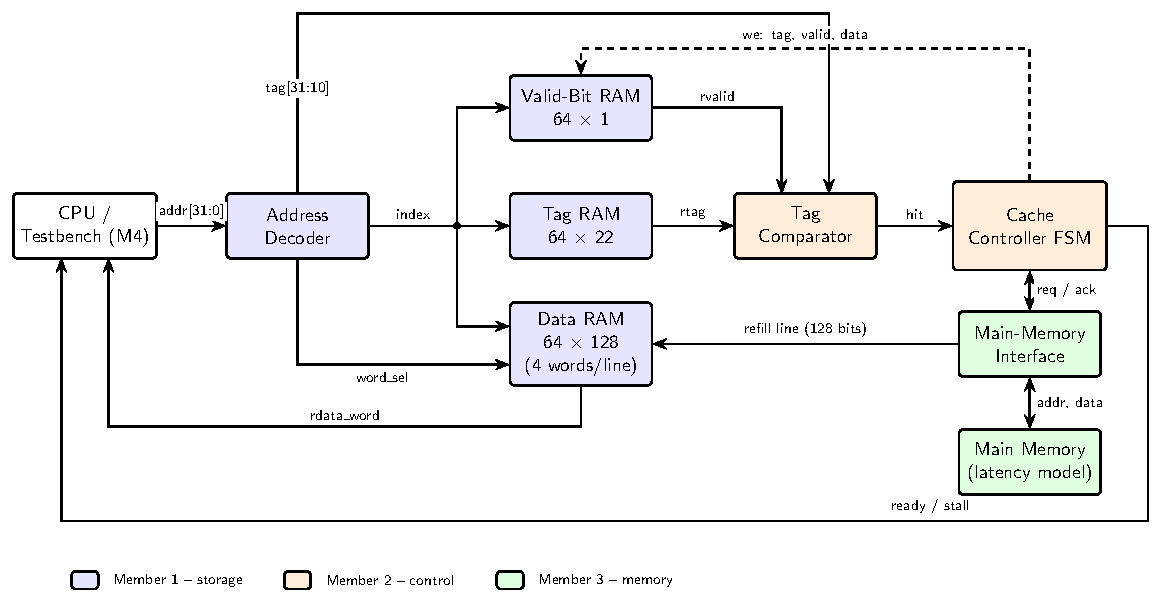
\includegraphics[width=0.9\textwidth]{figures/block_diagram.pdf}
\caption{Top-level block diagram of the direct-mapped cache. Shading shows
module ownership.}
\label{fig:block}
\end{figure*}

\subsubsection{Unit verification}
Each storage module has a self-checking Icarus Verilog testbench:
2012 field checks over random addresses for the decoder, 266 word
read-backs for the data RAM (including the partial-write and write-priority
cases), 68 for the tag RAM, and 196 for the valid bits (reset, flush and
reset-over-write priority). A storage-path test connects the decoder and the
three RAMs with the hit equation. It reproduces a cold miss, two spatial-locality
hits, a conflict miss at an address 1\,KB away that evicts the line, a
temporal-locality hit, and a miss after a flush. All tests pass, and Yosys
synthesis maps the storage to exactly the expected number of state bits.
% ----------------------- END PROPOSED SOLUTION A ----------------------


% -------------- REFERENCES (merge into the shared list) ---------------
% \begin{thebibliography}{9}
% \bibitem{smith1982} A.~J. Smith, ``Cache memories,'' \emph{ACM Computing
%   Surveys}, vol.~14, no.~3, pp.~473--530, Sep. 1982.
% \bibitem{hill1989} M.~D. Hill and A.~J. Smith, ``Evaluating associativity in
%   CPU caches,'' \emph{IEEE Trans. Computers}, vol.~38, no.~12,
%   pp.~1612--1630, Dec. 1989.
% \bibitem{jouppi1990} N.~P. Jouppi, ``Improving direct-mapped cache
%   performance by the addition of a small fully-associative cache and
%   prefetch buffers,'' in \emph{Proc. 17th Annu. Int. Symp. Computer
%   Architecture (ISCA)}, 1990, pp.~364--373.
% \bibitem{hennessy2017} J.~L. Hennessy and D.~A. Patterson, \emph{Computer
%   Architecture: A Quantitative Approach}, 6th~ed. Cambridge, MA, USA:
%   Morgan Kaufmann, 2017.
% \bibitem{patterson2020} D.~A. Patterson and J.~L. Hennessy, \emph{Computer
%   Organization and Design RISC-V Edition}, 2nd~ed. Morgan Kaufmann, 2020.
% \end{thebibliography}
 pieces into the IEEEtran report, or copy the
% blocks marked BEGIN/END. Figure path assumes the report lives in docs/.
% Citation keys used: smith1982, hill1989, jouppi1990, hennessy2017, patterson2020
% (bibitems at the bottom of this file -- merge into the shared reference list).
% =====================================================================

% ------------------------- BEGIN INTRODUCTION -------------------------
\section{Introduction}
Processor speeds have grown far faster than main-memory access times, so a
modern CPU would spend most of its cycles waiting on DRAM without a memory
hierarchy. A cache is a small, fast memory placed between the processor and
main memory. It keeps recently used blocks close to the processor and serves
most accesses in a single cycle. This works because real programs show
\emph{temporal locality} (a recently used address is likely to be used again
soon) and \emph{spatial locality} (addresses near a recently used one are
likely to be used next)~\cite{smith1982,hennessy2017}.

This project designs and verifies a parameterised direct-mapped cache
controller in Verilog. The default configuration is a 1\,KB cache with
16-byte blocks and 32-bit byte addresses. The design is split into storage
(data, tag and valid-bit RAMs and the address decoder), control (tag
comparator and controller FSM) and a main-memory interface. It is exercised
with sequential, repeated, random and conflict-heavy address traces, and
evaluated by hit ratio, miss ratio, average memory access time (AMAT) and
synthesis cost.
% -------------------------- END INTRODUCTION --------------------------


% ---------------------- BEGIN LITERATURE REVIEW A ---------------------
\subsection{Memory Hierarchy, Locality and Mapping Schemes}
Smith's survey of cache memories~\cite{smith1982} set out the main design
choices still used today: placement policy, block size, replacement and write
policy. It showed that small caches can achieve high hit ratios because of
program locality. The survey also showed that block size is a trade-off.
Larger blocks exploit spatial locality but raise the miss penalty, and in a
small cache they increase misses because fewer blocks fit.

Placement policy decides where a memory block may live in the cache. In a
\emph{direct-mapped} cache each block has exactly one possible line, chosen
by the index bits of the address. A \emph{fully associative} cache allows any
line, and an $n$-way \emph{set-associative} cache allows any of $n$ lines in
one set. Hill and Smith~\cite{hill1989} evaluated associativity with
trace-driven simulation and classified misses as compulsory, capacity and
conflict. Direct mapping suffers most from conflict misses, because two
frequently used blocks with the same index keep evicting each other. Its
advantage is that only one tag comparison is needed and no replacement
decision has to be made. This makes the hit path short and the hardware
small, so a direct-mapped cache can have a lower hit time than an associative
cache of the same size.

Jouppi~\cite{jouppi1990} kept the fast direct-mapped hit path and attacked
its conflict misses instead, by adding a small fully associative victim
cache that holds recently evicted lines. Textbook treatments by Hennessy and
Patterson~\cite{hennessy2017,patterson2020} combine these effects into a
single metric:
\begin{equation}
\mathrm{AMAT} = t_{\mathrm{hit}} + m \cdot t_{\mathrm{penalty}},
\end{equation}
where $m$ is the miss ratio. These sources motivate the design choices in
this project: direct mapping for a single-cycle hit and simple hardware, and
conflict-heavy traces to expose its main weakness.
% ----------------------- END LITERATURE REVIEW A ----------------------


% ---------------------- BEGIN PROPOSED SOLUTION A ---------------------
\subsection{Address Mapping and Cache Storage}

\subsubsection{Address breakdown}
For a cache of $C$ bytes with blocks of $B$ bytes and an $A$-bit address, the
number of lines and the field widths are
\begin{align}
N &= C/B, & b_{\mathrm{off}} &= \log_2 B,\\
b_{\mathrm{idx}} &= \log_2 N, & b_{\mathrm{tag}} &= A - b_{\mathrm{idx}} - b_{\mathrm{off}}.
\end{align}
With $C = 1024$, $B = 16$ and $A = 32$, this gives $N = 64$ lines, a 4-bit
offset (2 word-select bits and 2 byte bits), a 6-bit index and a 22-bit tag
(Table~\ref{tab:addr}). For example, address \texttt{0x12345678} decodes to
tag \texttt{0x048D15}, index 39 and word 2.

\begin{table}[t]
\centering
\caption{Address fields for the default configuration}
\label{tab:addr}
\begin{tabular}{lccc}
\hline
Field & Bits & Width & Selects \\
\hline
Tag      & [31:10] & 22 & Block identity \\
Index    & [9:4]   & 6  & One of 64 lines \\
Word     & [3:2]   & 2  & One of 4 words \\
Byte     & [1:0]   & 2  & Unused (word access) \\
\hline
\end{tabular}
\end{table}

The \texttt{address\_decoder} module is purely combinational. Its field
widths are Verilog parameters derived from \texttt{CACHE\_SIZE},
\texttt{BLOCK\_SIZE} and \texttt{ADDR\_WIDTH}, so the same RTL can be
re-targeted for the Phase~II parameter sweep without editing code. The unit
test checks both the default configuration and a 2\,KB / 32\,B configuration
(21/6/3/2 split).

\subsubsection{Storage organisation}
The cache state is held in three structures, all indexed by the same 6-bit
index (Fig.~\ref{fig:block}):
\begin{itemize}
  \item \textbf{Data RAM:} $64 \times 128$ bits (four 32-bit words per line,
        1\,KB). It supports a full-line write for refills and a single-word
        write for write hits. If both are requested, the line write takes
        priority.
  \item \textbf{Tag RAM:} $64 \times 22$ bits, written when a line is refilled.
  \item \textbf{Valid-bit array:} 64 bits, held as a register vector rather
        than a RAM so that a synchronous reset or flush clears every line in
        one cycle. After reset every access is a compulsory miss, even if a
        stale tag happens to match.
\end{itemize}
All three are read combinationally. The tag, valid bit and data for the
current index are therefore available in the same cycle, and the comparator
can compute $\mathit{hit} = \mathit{valid}[i] \wedge (\mathit{tag}[i] =
\mathit{addr}_{\mathrm{tag}})$ in a single cycle. The storage holds
$8192 + 1408 + 64 = 9664$ bits in total, so tag and valid bits add about 18\%
on top of the 8192 data bits.

\begin{figure*}[t]
\centering
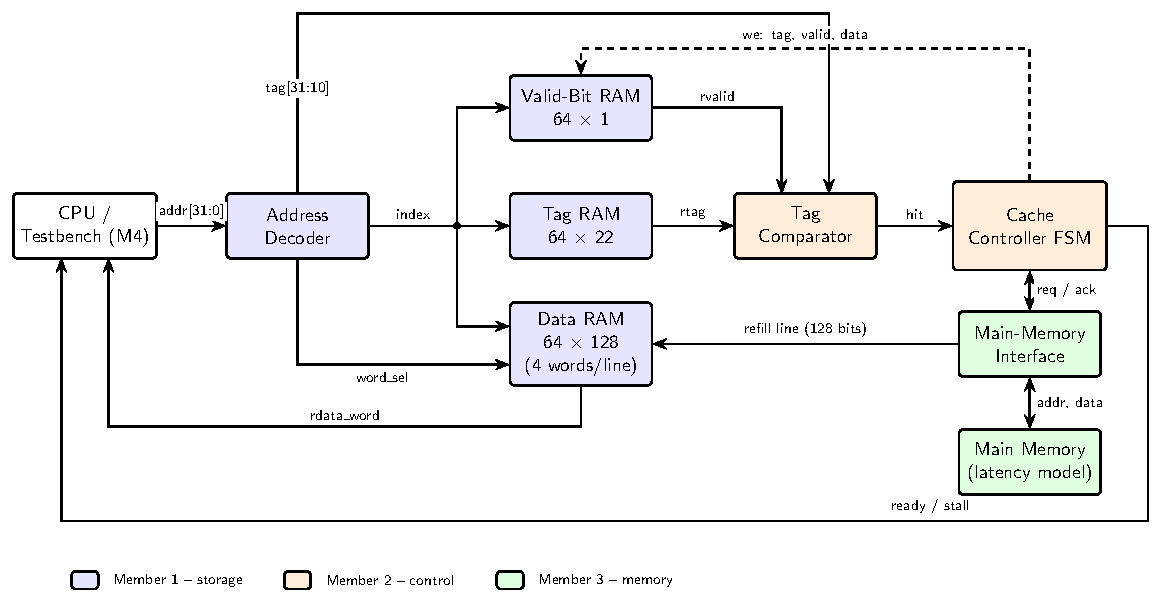
\includegraphics[width=0.9\textwidth]{figures/block_diagram.pdf}
\caption{Top-level block diagram of the direct-mapped cache. Shading shows
module ownership.}
\label{fig:block}
\end{figure*}

\subsubsection{Unit verification}
Each storage module has a self-checking Icarus Verilog testbench:
2012 field checks over random addresses for the decoder, 266 word
read-backs for the data RAM (including the partial-write and write-priority
cases), 68 for the tag RAM, and 196 for the valid bits (reset, flush and
reset-over-write priority). A storage-path test connects the decoder and the
three RAMs with the hit equation. It reproduces a cold miss, two spatial-locality
hits, a conflict miss at an address 1\,KB away that evicts the line, a
temporal-locality hit, and a miss after a flush. All tests pass, and Yosys
synthesis maps the storage to exactly the expected number of state bits.
% ----------------------- END PROPOSED SOLUTION A ----------------------


% -------------- REFERENCES (merge into the shared list) ---------------
% \begin{thebibliography}{9}
% \bibitem{smith1982} A.~J. Smith, ``Cache memories,'' \emph{ACM Computing
%   Surveys}, vol.~14, no.~3, pp.~473--530, Sep. 1982.
% \bibitem{hill1989} M.~D. Hill and A.~J. Smith, ``Evaluating associativity in
%   CPU caches,'' \emph{IEEE Trans. Computers}, vol.~38, no.~12,
%   pp.~1612--1630, Dec. 1989.
% \bibitem{jouppi1990} N.~P. Jouppi, ``Improving direct-mapped cache
%   performance by the addition of a small fully-associative cache and
%   prefetch buffers,'' in \emph{Proc. 17th Annu. Int. Symp. Computer
%   Architecture (ISCA)}, 1990, pp.~364--373.
% \bibitem{hennessy2017} J.~L. Hennessy and D.~A. Patterson, \emph{Computer
%   Architecture: A Quantitative Approach}, 6th~ed. Cambridge, MA, USA:
%   Morgan Kaufmann, 2017.
% \bibitem{patterson2020} D.~A. Patterson and J.~L. Hennessy, \emph{Computer
%   Organization and Design RISC-V Edition}, 2nd~ed. Morgan Kaufmann, 2020.
% \end{thebibliography}
 pieces into the IEEEtran report, or copy the
% blocks marked BEGIN/END. Figure path assumes the report lives in docs/.
% Citation keys used: smith1982, hill1989, jouppi1990, hennessy2017, patterson2020
% (bibitems at the bottom of this file -- merge into the shared reference list).
% =====================================================================

% ------------------------- BEGIN INTRODUCTION -------------------------
\section{Introduction}
Processor speeds have grown far faster than main-memory access times, so a
modern CPU would spend most of its cycles waiting on DRAM without a memory
hierarchy. A cache is a small, fast memory placed between the processor and
main memory. It keeps recently used blocks close to the processor and serves
most accesses in a single cycle. This works because real programs show
\emph{temporal locality} (a recently used address is likely to be used again
soon) and \emph{spatial locality} (addresses near a recently used one are
likely to be used next)~\cite{smith1982,hennessy2017}.

This project designs and verifies a parameterised direct-mapped cache
controller in Verilog. The default configuration is a 1\,KB cache with
16-byte blocks and 32-bit byte addresses. The design is split into storage
(data, tag and valid-bit RAMs and the address decoder), control (tag
comparator and controller FSM) and a main-memory interface. It is exercised
with sequential, repeated, random and conflict-heavy address traces, and
evaluated by hit ratio, miss ratio, average memory access time (AMAT) and
synthesis cost.
% -------------------------- END INTRODUCTION --------------------------


% ---------------------- BEGIN LITERATURE REVIEW A ---------------------
\subsection{Memory Hierarchy, Locality and Mapping Schemes}
Smith's survey of cache memories~\cite{smith1982} set out the main design
choices still used today: placement policy, block size, replacement and write
policy. It showed that small caches can achieve high hit ratios because of
program locality. The survey also showed that block size is a trade-off.
Larger blocks exploit spatial locality but raise the miss penalty, and in a
small cache they increase misses because fewer blocks fit.

Placement policy decides where a memory block may live in the cache. In a
\emph{direct-mapped} cache each block has exactly one possible line, chosen
by the index bits of the address. A \emph{fully associative} cache allows any
line, and an $n$-way \emph{set-associative} cache allows any of $n$ lines in
one set. Hill and Smith~\cite{hill1989} evaluated associativity with
trace-driven simulation and classified misses as compulsory, capacity and
conflict. Direct mapping suffers most from conflict misses, because two
frequently used blocks with the same index keep evicting each other. Its
advantage is that only one tag comparison is needed and no replacement
decision has to be made. This makes the hit path short and the hardware
small, so a direct-mapped cache can have a lower hit time than an associative
cache of the same size.

Jouppi~\cite{jouppi1990} kept the fast direct-mapped hit path and attacked
its conflict misses instead, by adding a small fully associative victim
cache that holds recently evicted lines. Textbook treatments by Hennessy and
Patterson~\cite{hennessy2017,patterson2020} combine these effects into a
single metric:
\begin{equation}
\mathrm{AMAT} = t_{\mathrm{hit}} + m \cdot t_{\mathrm{penalty}},
\end{equation}
where $m$ is the miss ratio. These sources motivate the design choices in
this project: direct mapping for a single-cycle hit and simple hardware, and
conflict-heavy traces to expose its main weakness.
% ----------------------- END LITERATURE REVIEW A ----------------------


% ---------------------- BEGIN PROPOSED SOLUTION A ---------------------
\subsection{Address Mapping and Cache Storage}

\subsubsection{Address breakdown}
For a cache of $C$ bytes with blocks of $B$ bytes and an $A$-bit address, the
number of lines and the field widths are
\begin{align}
N &= C/B, & b_{\mathrm{off}} &= \log_2 B,\\
b_{\mathrm{idx}} &= \log_2 N, & b_{\mathrm{tag}} &= A - b_{\mathrm{idx}} - b_{\mathrm{off}}.
\end{align}
With $C = 1024$, $B = 16$ and $A = 32$, this gives $N = 64$ lines, a 4-bit
offset (2 word-select bits and 2 byte bits), a 6-bit index and a 22-bit tag
(Table~\ref{tab:addr}). For example, address \texttt{0x12345678} decodes to
tag \texttt{0x048D15}, index 39 and word 2.

\begin{table}[t]
\centering
\caption{Address fields for the default configuration}
\label{tab:addr}
\begin{tabular}{lccc}
\hline
Field & Bits & Width & Selects \\
\hline
Tag      & [31:10] & 22 & Block identity \\
Index    & [9:4]   & 6  & One of 64 lines \\
Word     & [3:2]   & 2  & One of 4 words \\
Byte     & [1:0]   & 2  & Unused (word access) \\
\hline
\end{tabular}
\end{table}

The \texttt{address\_decoder} module is purely combinational. Its field
widths are Verilog parameters derived from \texttt{CACHE\_SIZE},
\texttt{BLOCK\_SIZE} and \texttt{ADDR\_WIDTH}, so the same RTL can be
re-targeted for the Phase~II parameter sweep without editing code. The unit
test checks both the default configuration and a 2\,KB / 32\,B configuration
(21/6/3/2 split).

\subsubsection{Storage organisation}
The cache state is held in three structures, all indexed by the same 6-bit
index (Fig.~\ref{fig:block}):
\begin{itemize}
  \item \textbf{Data RAM:} $64 \times 128$ bits (four 32-bit words per line,
        1\,KB). It supports a full-line write for refills and a single-word
        write for write hits. If both are requested, the line write takes
        priority.
  \item \textbf{Tag RAM:} $64 \times 22$ bits, written when a line is refilled.
  \item \textbf{Valid-bit array:} 64 bits, held as a register vector rather
        than a RAM so that a synchronous reset or flush clears every line in
        one cycle. After reset every access is a compulsory miss, even if a
        stale tag happens to match.
\end{itemize}
All three are read combinationally. The tag, valid bit and data for the
current index are therefore available in the same cycle, and the comparator
can compute $\mathit{hit} = \mathit{valid}[i] \wedge (\mathit{tag}[i] =
\mathit{addr}_{\mathrm{tag}})$ in a single cycle. The storage holds
$8192 + 1408 + 64 = 9664$ bits in total, so tag and valid bits add about 18\%
on top of the 8192 data bits.

\begin{figure*}[t]
\centering
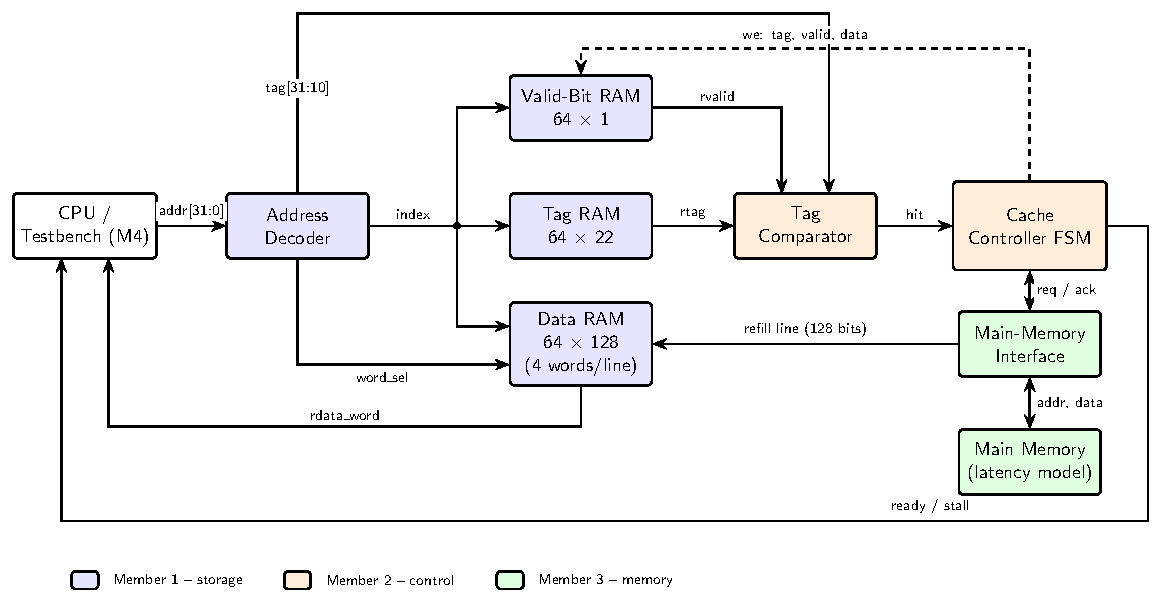
\includegraphics[width=0.9\textwidth]{figures/block_diagram.pdf}
\caption{Top-level block diagram of the direct-mapped cache. Shading shows
module ownership.}
\label{fig:block}
\end{figure*}

\subsubsection{Unit verification}
Each storage module has a self-checking Icarus Verilog testbench:
2012 field checks over random addresses for the decoder, 266 word
read-backs for the data RAM (including the partial-write and write-priority
cases), 68 for the tag RAM, and 196 for the valid bits (reset, flush and
reset-over-write priority). A storage-path test connects the decoder and the
three RAMs with the hit equation. It reproduces a cold miss, two spatial-locality
hits, a conflict miss at an address 1\,KB away that evicts the line, a
temporal-locality hit, and a miss after a flush. All tests pass, and Yosys
synthesis maps the storage to exactly the expected number of state bits.
% ----------------------- END PROPOSED SOLUTION A ----------------------


% -------------- REFERENCES (merge into the shared list) ---------------
% \begin{thebibliography}{9}
% \bibitem{smith1982} A.~J. Smith, ``Cache memories,'' \emph{ACM Computing
%   Surveys}, vol.~14, no.~3, pp.~473--530, Sep. 1982.
% \bibitem{hill1989} M.~D. Hill and A.~J. Smith, ``Evaluating associativity in
%   CPU caches,'' \emph{IEEE Trans. Computers}, vol.~38, no.~12,
%   pp.~1612--1630, Dec. 1989.
% \bibitem{jouppi1990} N.~P. Jouppi, ``Improving direct-mapped cache
%   performance by the addition of a small fully-associative cache and
%   prefetch buffers,'' in \emph{Proc. 17th Annu. Int. Symp. Computer
%   Architecture (ISCA)}, 1990, pp.~364--373.
% \bibitem{hennessy2017} J.~L. Hennessy and D.~A. Patterson, \emph{Computer
%   Architecture: A Quantitative Approach}, 6th~ed. Cambridge, MA, USA:
%   Morgan Kaufmann, 2017.
% \bibitem{patterson2020} D.~A. Patterson and J.~L. Hennessy, \emph{Computer
%   Organization and Design RISC-V Edition}, 2nd~ed. Morgan Kaufmann, 2020.
% \end{thebibliography}
 pieces into the IEEEtran report, or copy the
% blocks marked BEGIN/END. Figure path assumes the report lives in docs/.
% Citation keys used: smith1982, hill1989, jouppi1990, hennessy2017, patterson2020
% (bibitems at the bottom of this file -- merge into the shared reference list).
% =====================================================================

% ------------------------- BEGIN INTRODUCTION -------------------------
\section{Introduction}
Processor speeds have grown far faster than main-memory access times, so a
modern CPU would spend most of its cycles waiting on DRAM without a memory
hierarchy. A cache is a small, fast memory placed between the processor and
main memory. It keeps recently used blocks close to the processor and serves
most accesses in a single cycle. This works because real programs show
\emph{temporal locality} (a recently used address is likely to be used again
soon) and \emph{spatial locality} (addresses near a recently used one are
likely to be used next)~\cite{smith1982,hennessy2017}.

This project designs and verifies a parameterised direct-mapped cache
controller in Verilog. The default configuration is a 1\,KB cache with
16-byte blocks and 32-bit byte addresses. The design is split into storage
(data, tag and valid-bit RAMs and the address decoder), control (tag
comparator and controller FSM) and a main-memory interface. It is exercised
with sequential, repeated, random and conflict-heavy address traces, and
evaluated by hit ratio, miss ratio, average memory access time (AMAT) and
synthesis cost.
% -------------------------- END INTRODUCTION --------------------------


% ---------------------- BEGIN LITERATURE REVIEW A ---------------------
\subsection{Memory Hierarchy, Locality and Mapping Schemes}
Smith's survey of cache memories~\cite{smith1982} set out the main design
choices still used today: placement policy, block size, replacement and write
policy. It showed that small caches can achieve high hit ratios because of
program locality. The survey also showed that block size is a trade-off.
Larger blocks exploit spatial locality but raise the miss penalty, and in a
small cache they increase misses because fewer blocks fit.

Placement policy decides where a memory block may live in the cache. In a
\emph{direct-mapped} cache each block has exactly one possible line, chosen
by the index bits of the address. A \emph{fully associative} cache allows any
line, and an $n$-way \emph{set-associative} cache allows any of $n$ lines in
one set. Hill and Smith~\cite{hill1989} evaluated associativity with
trace-driven simulation and classified misses as compulsory, capacity and
conflict. Direct mapping suffers most from conflict misses, because two
frequently used blocks with the same index keep evicting each other. Its
advantage is that only one tag comparison is needed and no replacement
decision has to be made. This makes the hit path short and the hardware
small, so a direct-mapped cache can have a lower hit time than an associative
cache of the same size.

Jouppi~\cite{jouppi1990} kept the fast direct-mapped hit path and attacked
its conflict misses instead, by adding a small fully associative victim
cache that holds recently evicted lines. Textbook treatments by Hennessy and
Patterson~\cite{hennessy2017,patterson2020} combine these effects into a
single metric:
\begin{equation}
\mathrm{AMAT} = t_{\mathrm{hit}} + m \cdot t_{\mathrm{penalty}},
\end{equation}
where $m$ is the miss ratio. These sources motivate the design choices in
this project: direct mapping for a single-cycle hit and simple hardware, and
conflict-heavy traces to expose its main weakness.
% ----------------------- END LITERATURE REVIEW A ----------------------


% ---------------------- BEGIN PROPOSED SOLUTION A ---------------------
\subsection{Address Mapping and Cache Storage}

\subsubsection{Address breakdown}
For a cache of $C$ bytes with blocks of $B$ bytes and an $A$-bit address, the
number of lines and the field widths are
\begin{align}
N &= C/B, & b_{\mathrm{off}} &= \log_2 B,\\
b_{\mathrm{idx}} &= \log_2 N, & b_{\mathrm{tag}} &= A - b_{\mathrm{idx}} - b_{\mathrm{off}}.
\end{align}
With $C = 1024$, $B = 16$ and $A = 32$, this gives $N = 64$ lines, a 4-bit
offset (2 word-select bits and 2 byte bits), a 6-bit index and a 22-bit tag
(Table~\ref{tab:addr}). For example, address \texttt{0x12345678} decodes to
tag \texttt{0x048D15}, index 39 and word 2.

\begin{table}[t]
\centering
\caption{Address fields for the default configuration}
\label{tab:addr}
\begin{tabular}{lccc}
\hline
Field & Bits & Width & Selects \\
\hline
Tag      & [31:10] & 22 & Block identity \\
Index    & [9:4]   & 6  & One of 64 lines \\
Word     & [3:2]   & 2  & One of 4 words \\
Byte     & [1:0]   & 2  & Unused (word access) \\
\hline
\end{tabular}
\end{table}

The \texttt{address\_decoder} module is purely combinational. Its field
widths are Verilog parameters derived from \texttt{CACHE\_SIZE},
\texttt{BLOCK\_SIZE} and \texttt{ADDR\_WIDTH}, so the same RTL can be
re-targeted for the Phase~II parameter sweep without editing code. The unit
test checks both the default configuration and a 2\,KB / 32\,B configuration
(21/6/3/2 split).

\subsubsection{Storage organisation}
The cache state is held in three structures, all indexed by the same 6-bit
index (Fig.~\ref{fig:block}):
\begin{itemize}
  \item \textbf{Data RAM:} $64 \times 128$ bits (four 32-bit words per line,
        1\,KB). It supports a full-line write for refills and a single-word
        write for write hits. If both are requested, the line write takes
        priority.
  \item \textbf{Tag RAM:} $64 \times 22$ bits, written when a line is refilled.
  \item \textbf{Valid-bit array:} 64 bits, held as a register vector rather
        than a RAM so that a synchronous reset or flush clears every line in
        one cycle. After reset every access is a compulsory miss, even if a
        stale tag happens to match.
\end{itemize}
All three are read combinationally. The tag, valid bit and data for the
current index are therefore available in the same cycle, and the comparator
can compute $\mathit{hit} = \mathit{valid}[i] \wedge (\mathit{tag}[i] =
\mathit{addr}_{\mathrm{tag}})$ in a single cycle. The storage holds
$8192 + 1408 + 64 = 9664$ bits in total, so tag and valid bits add about 18\%
on top of the 8192 data bits.

\begin{figure*}[t]
\centering
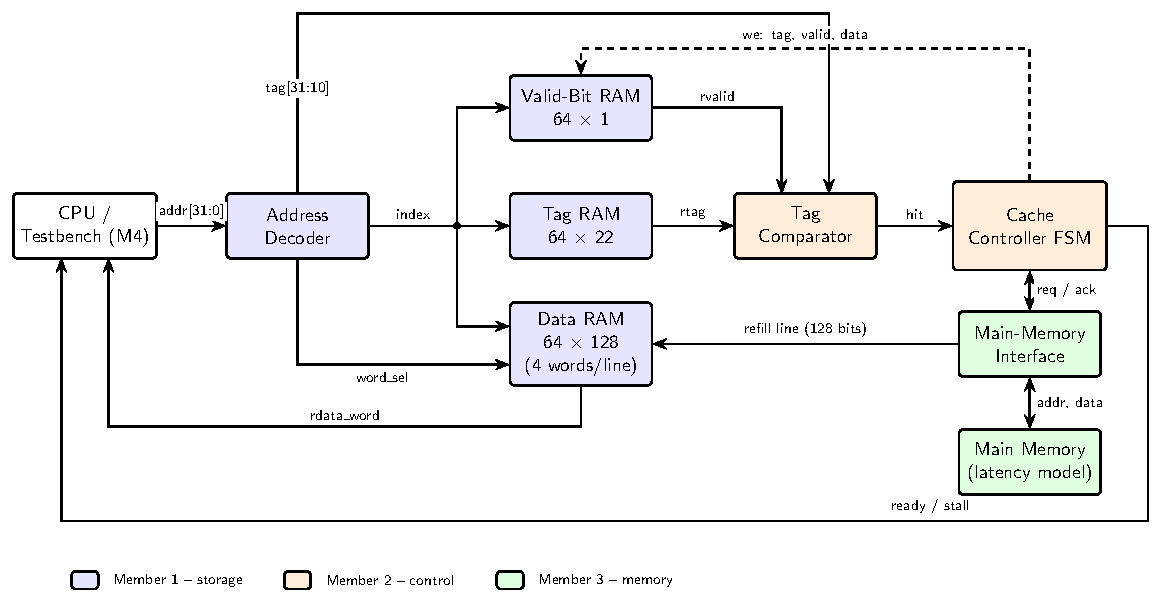
\includegraphics[width=0.9\textwidth]{figures/block_diagram.pdf}
\caption{Top-level block diagram of the direct-mapped cache. Shading shows
module ownership.}
\label{fig:block}
\end{figure*}

\subsubsection{Unit verification}
Each storage module has a self-checking Icarus Verilog testbench:
2012 field checks over random addresses for the decoder, 266 word
read-backs for the data RAM (including the partial-write and write-priority
cases), 68 for the tag RAM, and 196 for the valid bits (reset, flush and
reset-over-write priority). A storage-path test connects the decoder and the
three RAMs with the hit equation. It reproduces a cold miss, two spatial-locality
hits, a conflict miss at an address 1\,KB away that evicts the line, a
temporal-locality hit, and a miss after a flush. All tests pass, and Yosys
synthesis maps the storage to exactly the expected number of state bits.
% ----------------------- END PROPOSED SOLUTION A ----------------------


% -------------- REFERENCES (merge into the shared list) ---------------
% \begin{thebibliography}{9}
% \bibitem{smith1982} A.~J. Smith, ``Cache memories,'' \emph{ACM Computing
%   Surveys}, vol.~14, no.~3, pp.~473--530, Sep. 1982.
% \bibitem{hill1989} M.~D. Hill and A.~J. Smith, ``Evaluating associativity in
%   CPU caches,'' \emph{IEEE Trans. Computers}, vol.~38, no.~12,
%   pp.~1612--1630, Dec. 1989.
% \bibitem{jouppi1990} N.~P. Jouppi, ``Improving direct-mapped cache
%   performance by the addition of a small fully-associative cache and
%   prefetch buffers,'' in \emph{Proc. 17th Annu. Int. Symp. Computer
%   Architecture (ISCA)}, 1990, pp.~364--373.
% \bibitem{hennessy2017} J.~L. Hennessy and D.~A. Patterson, \emph{Computer
%   Architecture: A Quantitative Approach}, 6th~ed. Cambridge, MA, USA:
%   Morgan Kaufmann, 2017.
% \bibitem{patterson2020} D.~A. Patterson and J.~L. Hennessy, \emph{Computer
%   Organization and Design RISC-V Edition}, 2nd~ed. Morgan Kaufmann, 2020.
% \end{thebibliography}
